\paragraph{Experiment}
\begin{center}
	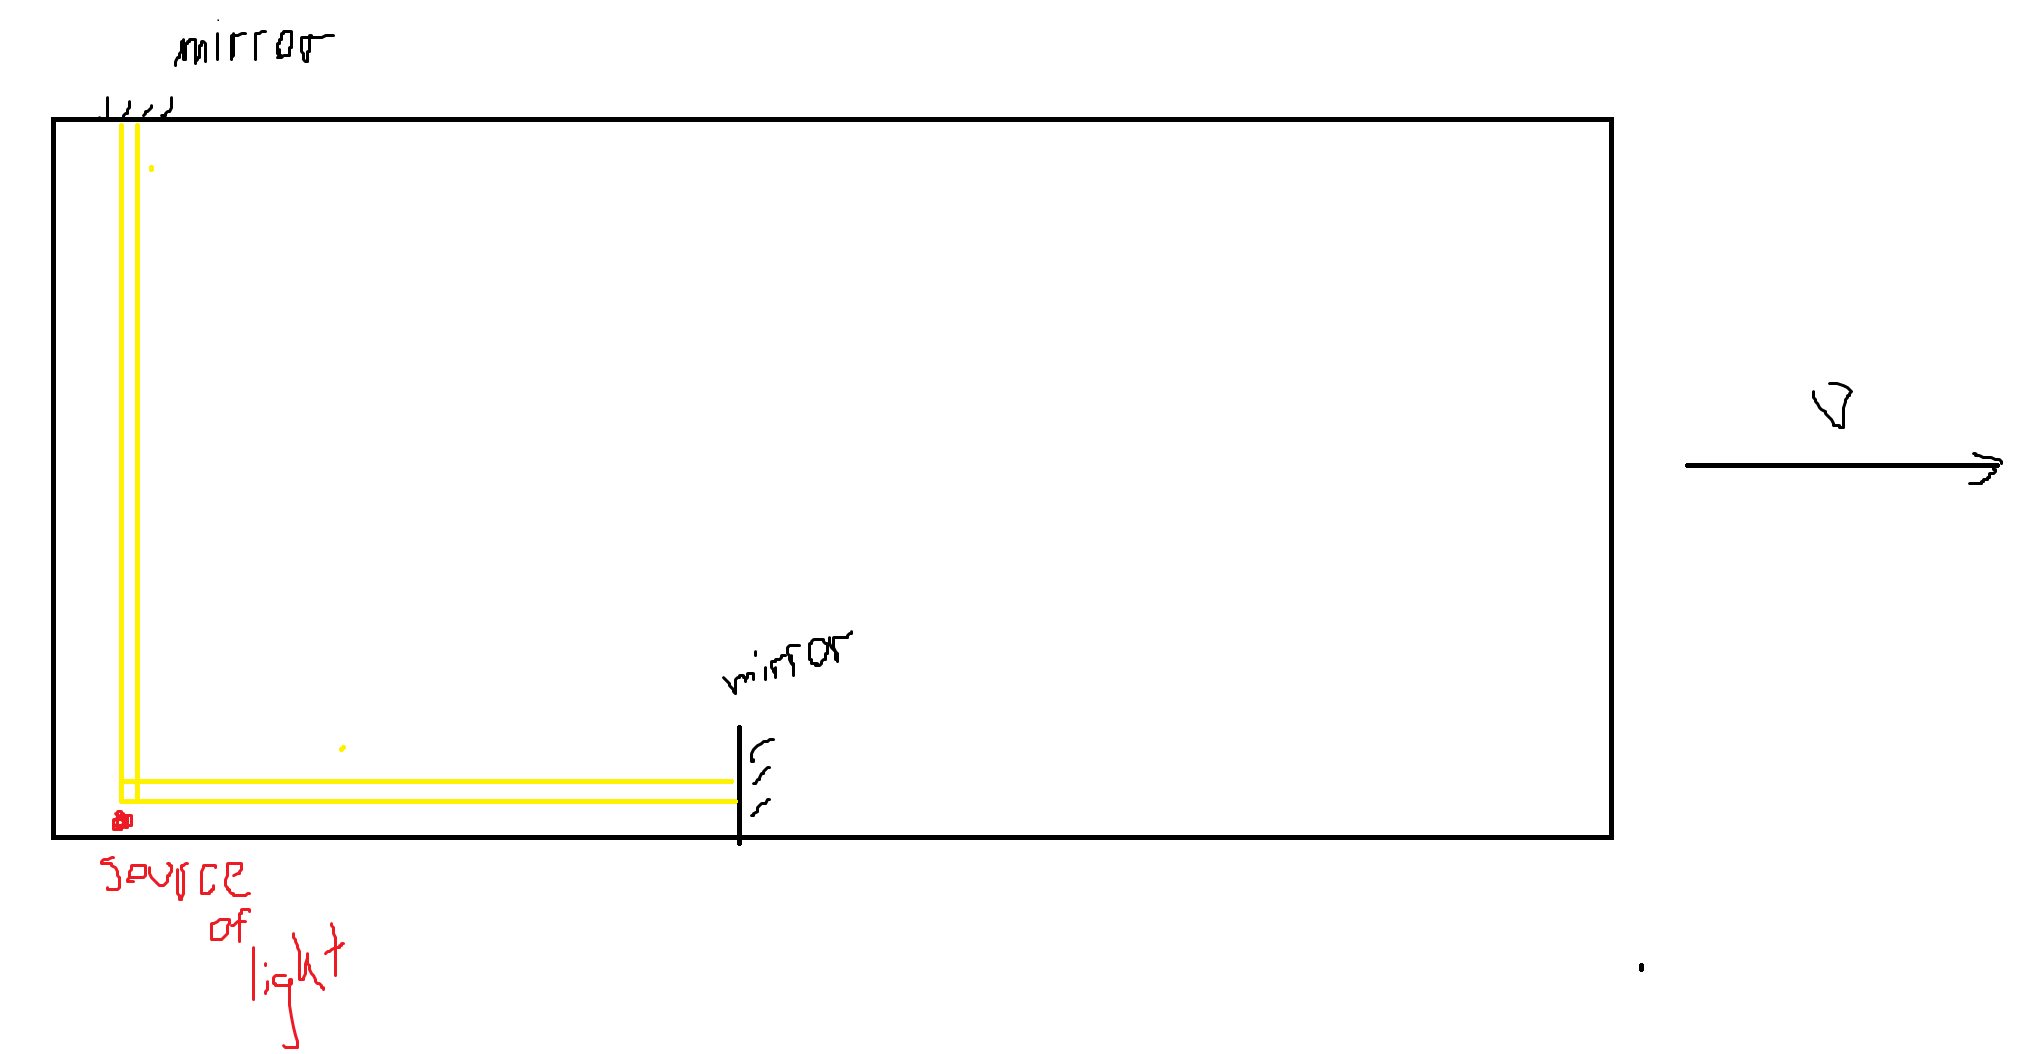
\includegraphics[width=\linewidth]{./lect21/pic1.png}
\end{center}

In Newtonian mechanics velocity of light would be $v+c$, but in relativity it's constant: $c$.

In frame of reference of lab, light passed $L+vt^\prime$. Then

$$ct^\prime = L+vt^\prime$$
$$t^\prime = \frac{L}{c-v}$$

When light returns from mirror, 

$$t^\prime_{back} = \frac{L}{c+v}$$

And total time according to lab:

$$t^\prime_{total} = \frac{L}{c-v} + \frac{L}{c+v} = \frac{2Lc}{c^2-v^2}= \frac{2\frac{L}{c}}{1-\frac{v^2}{c^2}}$$

From previous experiment:

$$t^\prime_{total} = \frac{t_0}{\sqrt{1-\frac{v^2}{c^2}}}$$

Putting all together:

$$\frac{2\frac{L}{c}}{1-\frac{v^2}{c^2}} = \frac{t_0}{\sqrt{1-\frac{v^2}{c^2}}}$$

Substituting $t_0 = \frac{2L_0}{c}$ we get:

$$L = \sqrt{1-\frac{v^2}{c^2}}L_0$$

\paragraph{Lorentz contraction}
Rod of length $L_0$ is resting in frame S. $L_0$ is a proper length (length in rest frame). Clock are synchronized at origin.

\subparagraph{Length measurements} We mark position of both ends of rod at some time $t^\prime$ (according to two different clocks in $S$):

$$\begin{cases*}
	x_1 = \gamma^\prime\left( x_1^\prime + vt^\prime \right)\\
	x_2 = \gamma^\prime\left( x_2^\prime + vt^\prime \right)
\end{cases*}$$

Acquiring

$$L_0 = x_2 - x_1 = \gamma^\prime \left( x_2^\prime - x_1^\prime \right)$$

\subsection{Relativity of simultaneity}
Let's write Lorentz transformation for both events:

$$t_1^\prime = =\gamma^\prime \left( t_1 - \frac{v}{c^2}x_1 \right)$$
$$t_2^\prime = =\gamma^\prime \left( t_2 - \frac{v}{c^2}x_2 \right)$$

Suppose $t_1^\prime = t_2^\prime$:

$$ \frac{v}{c^2}\left(x_2 - x_1\right) = t_2 - t_1 $$

So if $x_2>x_1$ then $t_2>t_1$, i.e. if in one frame of reference two events are simultaneous, in another frame of reference the "backward" event happens first.

\paragraph{Invariant}

$$\left(ct^\prime\right)^2 - \left({x^\prime}^2+{y^\prime}^2+{z^\prime}^2\right)=\left(ct \right)^2 - \left(x^2+y^2+z^2\right)$$

Lets substitute Lorentz transformation to the left side:

\begin{align*}
\left(ct^\prime\right)^2 - {x^\prime}^2 - {y^\prime}^2 - {z^\prime}^2 = \frac{\left(ct\right)^2 - 2tvx + \left(\frac{vx}{c}\right)^2}{1-\frac{v^2}{c^2}} - \frac{x^2 - 2tvx + v^2t^2}{1-\frac{v^2}{c^2}} - y^2-z^2 =\\= \left(ct\right)^2 \left[ \frac{1-\frac{v^2}{c^2}}{1-\frac{v^2}{c^2}} \right] - x^2\left[ \frac{1-\frac{v^2}{c^2}}{1-\frac{v^2}{c^2}} \right] - y^2 - z^2 = \left(ct \right)^2 - \left(x^2+y^2+z^2\right)
\end{align*}

If $\left(c\Delta t\right)^2 - \left(\Delta x\right)^2 - \left(\Delta y\right)^2 - \left(\Delta z\right)^2 < 0$ then events switch their order, and no information can pass from one to the other.